\documentclass[bigger]{beamer}

\mode<presentation>
{
  \usetheme{default}
  \usecolortheme{crane}
  \usefonttheme{serif}
  \setbeamercovered{transparent}
%--------------------------------------------------
%   \setbeamerfont{small}{size=\small}
%-------------------------------------------------- 
}

\usepackage[english]{babel}
\usepackage{times}
\usepackage{algorithmic}
\usepackage{algorithm}
\usepackage{epsfig}
% Latin-1 only
\usepackage[latin1]{inputenc}
\usepackage[T1]{fontenc}
%--------------------------------------------------
% % Chinese-support
% \usepackage[nocjkbg5]{ucs}
% \usepackage[utf8x]{inputenc}
% \usepackage[C00,T1]{fontenc}
% \newcommand\tradtext[1]{\bgroup\fontencoding{C00}\fontfamily{ming}\selectfont%
% \SetUnicodeOption{cjkbg5}#1\egroup}
%-------------------------------------------------- 

\title[]
{Paper Survey}
\subtitle[]
{Abhinandan Das, Mayur Datar, Ashutosh Garg, Shyam Rajaram. ``Google News Personalization: Scalable Online Collaborative Filtering.''  WWW 2007}
\author[] % (optional, use only with lots of authors)
{Ruey-Cheng Chen}
\institute % (optional, but mostly needed)
{Academia Sinica, Taiwan}
\date[] % (optional, should be abbreviation of conference name)
{May 15, 2007}
\subject{Theoretical Computer Science}
% \pgfdeclareimage[height=0.5cm]{university-logo}{university-logo-filename}
% \logo{\pgfuseimage{university-logo}}
%--------------------------------------------------
% \AtBeginSubsection[]
% {
%   \begin{frame}<beamer>
%     \frametitle{Outline}
%     \tableofcontents[currentsection,currentsubsection]
%   \end{frame}
% }
%-------------------------------------------------- 
%\beamerdefaultoverlayspecification{<+->}
\newcommand<>\info[2]{\begin{block}{#1}#2\end{block}}
\newcommand\newblock[2]{\newcommand<>{#1}[1]{\info{#2}{##1}}}
\newblock{\algo}{Algorithm}
\newblock{\proc}{Procedure}
\newblock{\idea}{Idea}
\newblock{\reference}{Reference}
\newcommand<>\ul[1]{\begin{itemize}#1\end{itemize}}
\newcommand<>\ol[1]{\begin{enumerate}#1\end{enumerate}}
\newcommand<>\dl[1]{\begin{description}#1\end{description}}

\begin{document}

\frame{ \titlepage }
\frame{ \frametitle{Outline} \large \tableofcontents }

%--------------------------------------------------
% \section{Introduction}
% \frame{
%   \frametitle{Introduction}
% }
%-------------------------------------------------- 

\section{Problem Setting}
\frame{
  \frametitle{Problem Setting}
  
  Problem Statement
  \ul{
    \item Presented with the click history for $N$ users ($U = \{
      u_1,u_2,\ldots,u_N \}$) over $M$ items ($S = \{ s_1,s_2,\ldots,s_M \}$),
      and given a specific user $u$ with click history set $C_u$ consisting of
      stories $\{ s_{i_1},\ldots,s_{i_{|C_u|}} \}$, recommend $K$ stories to
      the user that she might be interested in reading.
  }

  Challenges
  \ul{
    \item Large-scale operations (e.g., adding/dropping news stories every few minutes)
    \item Strict response time requirement (for any page views)
    \item Binary ratings (as opposed to 1-5 star ratings)
  }
}

\section{Related Work}

\frame{
  \frametitle{Related Work}
  Memory-Based Algorithms
  \ul{
    \item The prediction is calculated as a weighted average of the ratings
    given by other users, where the weight is proportional to the simlarity
    between users, as in: \begin{displaymath}r_{u_a,s_k} = \sum_{i \neq
    a}\limits I_{(u_i,s_k)}w(u_a,u_i)\end{displaymath} where $I_{(u_i,s_k)}$ is
    the indicator variable

    \item Commonly used similarity measures includes:
    \ul{
      \item The Pearson correlation coefficient \cite{resnick:goa}
      \item Cosine similarity \cite{breese1998eap}
    }
    \item Cons: Scalability 
    \ul{\item All-pair computation is infeasible}
  }
}

\frame{
  \frametitle{Related Work (cont'd)}
  Model-Based Algorithms
  \ul{
    \item Cluster models
    \ul{\item Capturing user interests \item Reducing dimensions}
    \item Approaches
    \ul{
      \item LSI \cite{sarwar2000adr}
      \item Bayesian Clustering \cite{breese1998eap}
      \item PLSI \cite{hofmann2004lsm}
      \item Multiple Multiplicative Factor Model \cite{marlin2004mmf}
      \item Markov Decision Process %\cite{shani2005mbr}
      \item Latent Dirichlet Allocation \cite{blei2003lda}
    }
  }

}

\section{Algorithms}
\frame{
  \frametitle{Algorithms}

  A Mix of Algorithms
  \ul{
    \item MinHash
    \item PLSI
    \item Covisitation
  }

  Score $r_{u_a,s_k}$
  \ul{

    \item For \emph{clustering approaches}, the score is proportional to
    \begin{displaymath}r_{u_a,s_k} \varpropto \sum_{c_i:u_a \in c_i}\limits
    w(u_a,c_i) \sum_{u_j:u_j \in c_i}\limits I_{(u_j,s_k)}\end{displaymath}
    where $w(u_a,c_i)$ is proportional to the fractional membership of the user
    $u_a$ to cluster $c_i$

    \item For the covisitation method, the score is proportional to the number
    of times the story was covisited with the other (stories)

  }
}

\subsection{MinHash}
\frame{
  \frametitle{MinHash}
  
  Basic Idea
  \ul{
    \item Representing a user $u$ by her click history $C_u$
    \item Using Jaccard coefficient as the similarity measure
    \begin{displaymath}S(u_i,u_j) = \frac{|C_{u_i} \cap C_{u_j}|}{|C_{u_i} \cup C_{u_j}|}\end{displaymath}
    \item Pruning search space by using Locality Sensitive Hashing (LSH) \cite{indyk1998ann}
    \ul{
      \item To hash the data points using several hash functions so as to
      ensure that, for each function, the probability of collision is much
      higher for objects which are close to each other than for those which are
      far apart
    }
  }
}

\frame{
  \frametitle{MinHash (cont'd)}
  MinHashing \cite{cohen1997sef}
  \ul{
    \item Permuting the set of items $S$ randomly
    \item Computing hash value $h(u_i)$ as the index of the \emph{first} item
    under the permutation that belongs to $C_u$
    \ul{\item The probability of collision is exactly equal to Jaccard
    coefficient \cite{cohen1997sef,broder1997rac,cohen2001fia}}
    \item Concatenating $p$ ($p > 1$) hash-keys for users to improve within-cluster similarity
    \ul{\item The probability of collision is equal to $S(u_i,u_j)^p$}
    \item Using MapReduce \cite{dean:msd}
    \ul{\item Map inputs to key-value pairs \item Partition and shuffle the key-value pairs \item Reduce key-value pairs}
  }
}

\subsection{PLSI}
\frame{
  \frametitle{PLSI}
  Probabilistic Latent Semantic Model \cite{hofmann2004lsm}
  \ul{
    \item The mixture model is \begin{displaymath}p(s|u;\theta) =
    \sum_{z=1}^L\limits p(z|u)p(s|z)\end{displaymath} where the latent variable
    $z \in Z$ ($\lVert Z \rVert = L$) representing user communities and item
    communities is introduced

    \item EM algorithm is revised to work with MapReduce
    \item Can PLSI work online?
    \ul{
      \item $P(s|z)$ can be updated in real time (approximately)
      \item The model should be rebuilt whenever $P(z|u)$ changes (new users cannot be added)
      \item Parallelizing will not solve the problem
    }
  }
}

%--------------------------------------------------
% \subsection{User Clustering}
%-------------------------------------------------- 

\subsection{Covisitation}
\frame{
  \frametitle{Covisitation}
  Covisitation
  \ul{
    \item An event in which two stories are clicked by the same user within a
    certain time interval (e.g., a few hours)
    \item ``Users who viewed this item also viewed the following items''
  }
  Adjacency lists in a Bigtable \cite{chang2006bds}
  \ol{
    \item Retriving $C_{u_i}$ and iterate over items in it (when user $u_i$ click on item $s_k$) 
    \item Modifying the adjacency lists for both $s_j \in C_{u_i}$ and $s_k$ to add an entry
    \item Updating the age discounted count (when an entry is there already)
  }
  Computation of the score $r_{u_i,s}$ for user $u_i$
  \ol{
    \item Looking up the entry for $s_i \in C_{u_i}$ and $s$ 
    \item Normalizing the scores by linear scaling
  }
}

%--------------------------------------------------
% \subsection{Candidate Generation}
%-------------------------------------------------- 

\section{System Setup}
\frame{
  \frametitle{System Setup}
  Components
  \ul{
    \item User Table \textbf{UT}
    \item Story Table \textbf{ST}
    \item News Statistics Server \textbf{NSS}
    \item News Front-End \textbf{NFE}
    \item News Personalization Server \textbf{NSE}
  }

  \begin{figure}
    \centering
    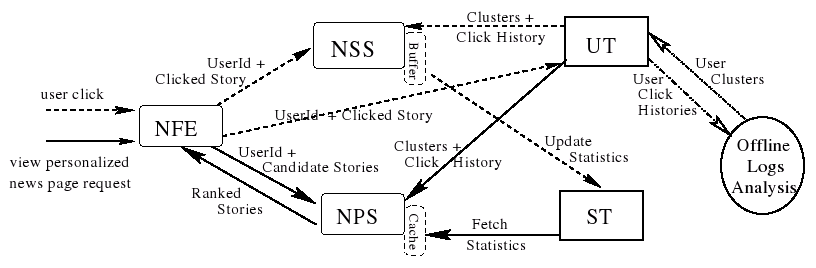
\includegraphics[width=\columnwidth]{component}
  \end{figure}
}

\section{Evaluation}

\frame{
  \frametitle{Evaluation}
  Setup
  \ul{
    \item Datasets: MovieLens, NewsSmall, NewsBig
    \item Training/Test: 80\%/20\% (for each user)
  }
  Algorithms
  \ul{
    \item MinHash: each user is classified into 100 clusters
    \item Correlation: all-pair computation with cosine similarity
    \item PLSI
  }
  Output
  \ul{
    \item The inferred rating is in $[0,1]$ and is binarized to 1 if it exceeds
    a certain threshold, 0 otherwise
    \item The threshold is chosen from the set $\{10^{-x}|x \in \{0.1,0.2,\ldots,4\}\}$
  }
}

\frame{
  \frametitle{Results: MovieLens}
  Movie rating data (collected using a recommender system)
  \ul{
    \item 943 users, 1,670 movies, and about 54,000 ratings (binarized from 1-5 star ratings)
  }
  \begin{figure}
    \centering
    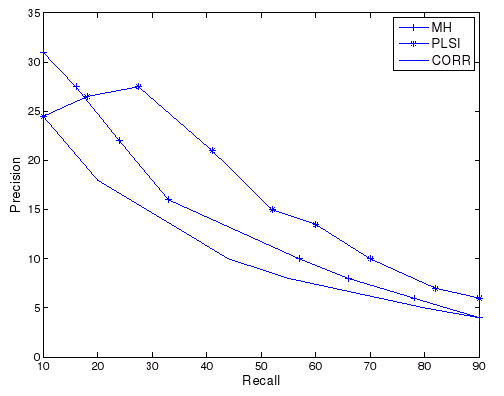
\includegraphics[width=200pt]{eval1}
    \caption{Precision-Recall curves for the MovieLens dataset}
  \end{figure}
}

\frame{
  \frametitle{Results: NewsSmall and NewsBig}
  Two subsets of Google News clickstream
  \ul{
    \item 5,000/500,000 users, 40,000/190,000 items, and 370,000/10,000,000 clicks
  }
  \begin{figure}
    \centering
    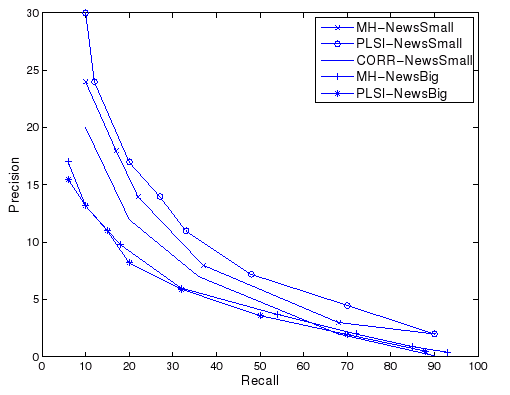
\includegraphics[width=200pt]{eval2}
    \caption{Precision-Recall curves for the Google News datasets}
  \end{figure}
}

\frame{
  \frametitle{Evaluation on Live Traffic}
  Comparison between different algorithms
  \ul{
    \item Popular (age discounted click count)
  }
  \begin{figure}
    \centering
    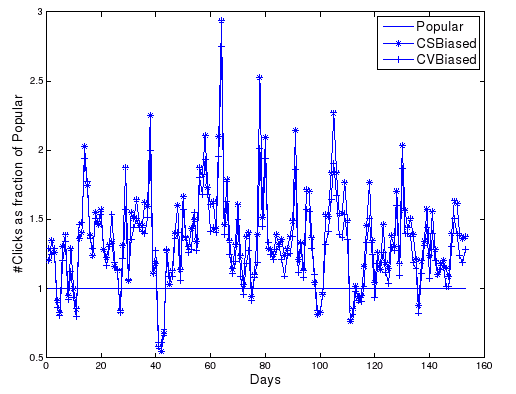
\includegraphics[width=200pt]{eval3}
    \caption{Live traffic click ratios (with baseline as Popular algorithm)}
  \end{figure}
}

\frame{
  \frametitle{Evaluation on Live Traffic (cont'd)}
  Comparison between MinHash and PLSI
  \begin{figure}
    \centering
    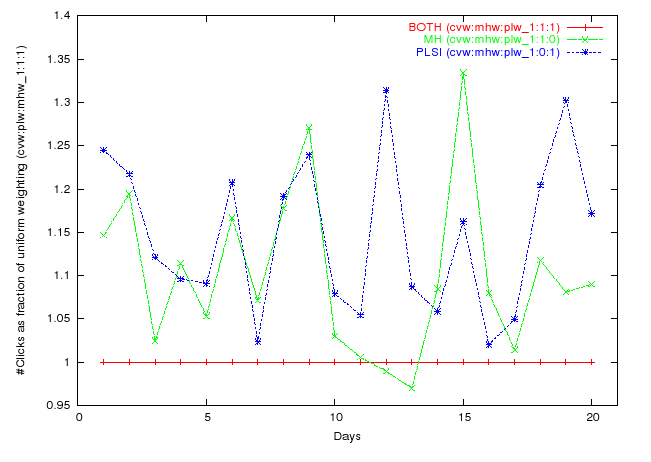
\includegraphics[width=230pt]{eval4}
    \caption{Live traffic click ratios (with baseline as Popular algorithm)}
  \end{figure}
}

\section{Conclusion}
\frame{
  \frametitle{Conclusion}
  Contributions
  \ul{
    \item Presenting the algorithms behind a scalable real-time recommendation engine
    \item Presenting novel approaches to clustering over dynamic datasets using MinHash and PLSI
    \item Adapting methods to the MapReduce framework
    \item Showing that the scalability does not come at the cost of quality
  }
  Future Work
  \ul{
    \item Learning techniques
    \item Higher order covisitation statistics
  }
}

%--------------------------------------------------
% \section{Discussion}
% \frame{
%   \frametitle{Discussion}
% }
%-------------------------------------------------- 

% All of the following is optional and typically not needed. 
\appendix
\section<presentation>*{\appendixname}

\begin{frame}[allowframebreaks]
  \frametitle{Reference}
  \begin{scriptsize}
    \bibliography{slides}
    \bibliographystyle{alpha}
  \end{scriptsize}
\end{frame}

\frame{
  \center
  \begin{tabular}{c}
    \Huge{Thanks for Your Attension!}\\
    \\
    \large{Any Questions?}
  \end{tabular}
}

\end{document}
